\documentclass{beamer}

\usepackage[utf8]{inputenc}
\usepackage[russian]{babel}
\usepackage{latexsym}
\usepackage{hyperref}

\title[Поверхность молекулы]{Поверхность молекулы и поверхность
    контакта молекул: зачем нужны, алгоритмы, сервисы, примеры применения}
\date{2012}
\usetheme{Warsaw}
\usecolortheme{seahorse}

\begin{document}
    \begin{frame}
        \titlepage
    \end{frame}

    \begin{frame}{Цели построения молекулярной поверхности}
        \begin{itemize}
        \item Для вычисления площади поверхности
         % Площадь поверхности контакта двух молекул позволяет оценить
         % их взаимодействие и, следовательно, стабильность комплекса
        \item Для визуализации на поверхности электростатического потенциала,
            гидрофобных областей и других характеристик
         % Помогает предсказывать области белка, взаимодействующие с
         % другими молекулами, проверять корректность моделей
        \item Для выявления полостей, каналов в белке, карманов и т.п.
         % Следовательно, доступных для воды, ионов, лигандов
        \item Для выявления остатков, экспонированных на поверхности белка
         % Если в одном белке область важна для взаимодействия с
         % другой молекулой, то для похожей области в другом белке
         % можно предсказать подобное же взаимодействие
        \item Для поиска сходных областей поверхности
         % расчет энергии сольватации,  симуляция молекулярной динамики, докинг
        \item \dots
        \end{itemize}
    \end{frame}

    \begin{frame}{Типы молекулярной поверхности}
        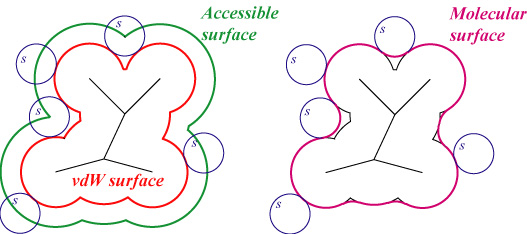
\includegraphics[width=\linewidth]{types.jpg}
        \begin{itemize}
        \item vdWS: Ван-дер-Ваальсова
        \item SAS: доступная для воды
        \item MS: поверхность Коннолли
        \end{itemize}
    \end{frame}

    \begin{frame}{Ван-дер-Ваальсовы радиусы (\AA) для атомов
        некоторых элементов (по Ли и Ричардсу)}
        \begin{tabular}{ l l }
            S & 1.80 \\
            P & 1.80 \\
            O & 1.52 \\
            N & 1.55 \\
            C & 1.70 \\
            H & 1.20 \\
        \end{tabular}
    \end{frame}

    \begin{frame}{Типы молекулярной поверхности}{vdWS: Ван-дер-Ваальсова}
        \includegraphics[trim=2cm 5cm 2cm 5cm, clip, width=\linewidth]{vdw.png}

        состоит из точек, лежащих на Ван-дер-Ваальсовах сферах атомов молекулы и
        не попадающих внутрь Ван-дер-Ваальсовых сфер других атомов.

        Может содержать сквозные просветы (смотри на рисунке слева).
    \end{frame}

    \begin{frame}{Типы молекулярной поверхности}{SAS: доступная для воды}
        \includegraphics[trim=2cm 5cm 2cm 5cm, clip, width=\linewidth]{sas.png}

        описана центром сферической молекулы воды (радиус 1.4 \AA),
        <<прокатанной>> вокруг атомов белка.

        % Поверхность, доступная для воды, использовалась, например, для того,
        % чтобы показать, какие аминокислотные остатки чаще экспонированы --
        % доступны для воды
    \end{frame}

    \begin{frame}{Типы молекулярной поверхности}{SAS: доступная для воды}
        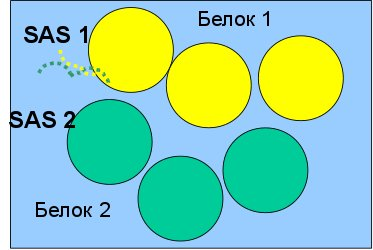
\includegraphics[width=0.5\linewidth]{sas-contact.jpg}

        SAS не подходит для изучения поверхности контакта двух белков
        из-за перекрывания поверхностей белков.
    \end{frame}

    \begin{frame}{Типы молекулярной поверхности}{MS: поверхность Коннолли}
        \includegraphics[trim=2cm 5cm 2cm 5cm, clip, width=\linewidth]{connolly.png}

        описана поверхностями молекул воды, находящимися в контакте с белком;

        <<поверхность, исключаемая растворителем>>:
        поверхность тела, получающегося при исключении из объема точек,
        в которых может находиться растворитель.
    \end{frame}

    \begin{frame}{Поверхность молекулы (Connolly surface)}
        Состоит из двух частей:
        \begin{itemize}
        \item \emph{Поверхность контакта} образована точками ван-дер-ваальсовых
            сфер атомов белка, которых может коснуться ван-дер-ваальсова сфера
            молекулы воды.
        \item \emph{Дополнительная поверхность} образована поверхностью
            молекул воды, касающихся белка в \emph{двух} или \emph{трех} точках.
        \end{itemize}
    \end{frame}

    \begin{frame}{Поверхность молекулы (Connolly surface)}
        Состоит из участков трёх видов:
        \begin{itemize}
        \item \emph{Выпуклые сферы}, совпадающие с поверхностью контакта.
        \item \emph{Выгнутые сферы}, относящиеся к дополнительной поверхности,
            образуются при контакте молекулы воды одновременно с \emph{тремя}
            точками белка.
        \item \emph{Тороидальные участки},
            относящиеся к дополнительной поверхности,
            образуются при заметании подвижным шариком молекулы воды,
            который вращается между \emph{двумя} фиксированными шарами
            (группами белка) все время касаясь обоих.
        \end{itemize}
    \end{frame}

    \begin{frame}{Поверхность молекулы (Connolly surface)}
        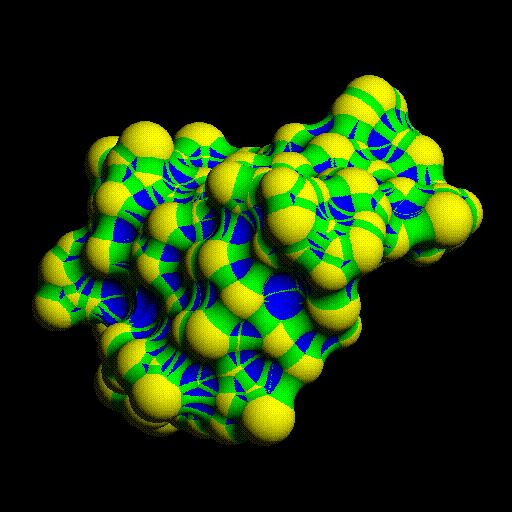
\includegraphics[height=0.9\textheight]{connolly-types.jpg}
    \end{frame}

    \begin{frame}{Поверхность молекулы (Connolly surface)}{Вогнутые сферы}
        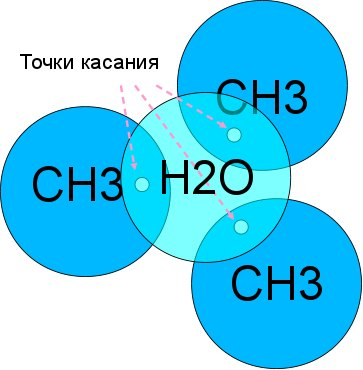
\includegraphics[height=0.7\textheight]{connolly-3-points.jpg}
    \end{frame}

    \begin{frame}{Поверхность молекулы (Connolly surface)}{Тороидальные участки}
        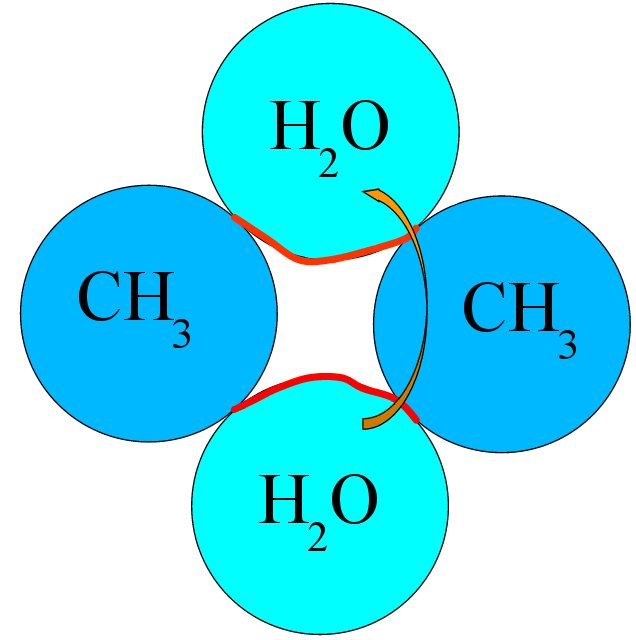
\includegraphics[height=0.7\textheight]{connolly-2-points.jpg}
    \end{frame}

    \begin{frame}{Основные алгоритмы построения поверхности и вычисления её площади}
        \begin{itemize}
        \item \emph{Приближенные аналитические} \\
            (Richards and Lee, 1971; Wodak and Janin, 1980)
        \item \emph{Представление поверхности точками} \\
            (Shrake and Rupley, 1973; Connolly, 1983)
        \item \emph{Точные аналитические методы} \\
            (Gibson and Scheraga, 1987;  Richmond, 1984)
        \end{itemize}
    \end{frame}

    \begin{frame}{Метод срезов Ли -- Ричардса
        для вычисления площади SAS}
        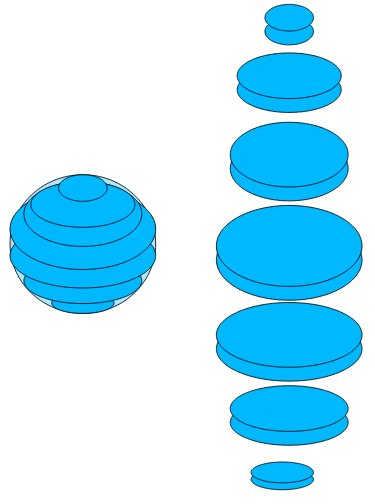
\includegraphics[height=0.7\textheight]{lee.jpg}
    \end{frame}

    \begin{frame}{Метод срезов Ли -- Ричардса
        для вычисления площади SAS}
        \begin{itemize}
        \item Создается серия параллельных срезов,
            находящихся на фиксированном расстоянии друг от друга.
        \item Для каждого среза находятся <<круги>> от атомов.
        \item Вычисляется длина границы.
        \item Умножается на расстояние между срезами.
        \item Берется сумма по всем срезам
        \end{itemize}
    \end{frame}

    \begin{frame}{Метод точечной поверхности Коннолли}
        \begin{itemize}
        \item Поверхность представлена точками:
            \begin{itemize}
            \item Поверхность контакта
             % на поверхности каждой VdW сферы атома белка строится
             % равномерная сеть точек;
             % для каждой точки проверяется, что молекула воды,
             % касающаяся этой точки, не пересекается с белком;
             % если пересекается, то точка удаляется.
            \item Дополнительная поверхность -- тороидальная
             % Каждая пара соседних атомов определяет тороидальную поверхность
             % между ними
             % На этой поверхности строится равномерная сеть точек
             % Далее – как для контактной поверхности
            \item Дополнительная поверхность -- сферическая
             % Каждая тройка соседних атомов определяет сферическую
             % дополнительную поверхность -- ван-дер-ваальсову поверхность
             % молекулы воды, касающейся этих атомов
             % Если эта молекула воды не пересекается с белком, то на
             % подходящей части этой поверхности строится равномерная сеть точек
            \end{itemize}
        \item Число отобранных точек пропорционально площади поверхности белка
        \item На этих точках может быть построена триангуляция поверхности для
            визуализации (или более точного подсчета площади)
        \end{itemize}
    \end{frame}

    \begin{frame}{Алгоритм Shrake-Rupley}
        \begin{itemize}
        \item Вокруг каждого атома на расстоянии, равном сумме Ван-дер-Ваальсова
            радиуса и радиуса молекулы воды, создается равномерная сеть точек.
        \item Для каждой точки проверяется, <<утоплена>> ли она в окружающих
            атомах или является доступной для растворителя.
        \item Число отобранных точек пропорционально площади поверхности белка
        \end{itemize}
    \end{frame}

    \begin{frame}{Влияние параметров на результат}{На примере Shrake-Rupley}
        \begin{itemize}
            \item радиус молекулы растворителя \\
                (уменьшение приводит к увеличению результата)
            \item Ван-дер-Ваальсовы радиусы атомов
                \begin{itemize}
                \item Наличие водородов в структуре (если нет -- их радиус может
                    быть неявно учтен в радиусах атомов остальных элементов)
                \end{itemize}
            \item Количество точек, создаваемое на каждой сфере \\
                (увеличение приводит к повышению уровня детализации)
        \end{itemize}
    \end{frame}

    \begin{frame}{Аналитический метод определения площади поверхности
        (Kratky, 1981)}
        \begin{itemize}
            \item Площадь $S_A$ vdW сферы атома A равна $4\pi r^2$
            \item Нужно найти площадь $(S_A)_0$  области, не попадающей внутрь
                vdW сфер других атомов; тогда $S=\sum\limits_A (S_A)_0$.
            \item Для двух пересекающихся сфер площадь $S_{A,B}$
                области на 1-й сфере, попадающей внутрь 2й, вычисляется
                (в зависимости от радиусов и расстояния между центрами).
            \item Также может быть вычислена площадь
                более сложных пересечений и, следовательно, $(S_A)_0$.
        \end{itemize}
    \end{frame}

    \begin{frame}{Поверхность контакта двух молекул A и B}
        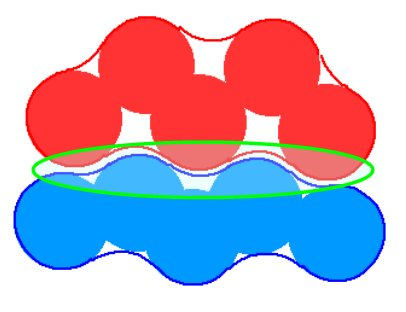
\includegraphics[height=0.4\textheight]{contact.jpg}

        $$ S_{cont} = \frac{S_A + S_B - S_{A \cup B}}{2} $$
         % вклад взаимодействия макромолекул (или частей макромолекул)
         % в энергию системы примерно пропорционален площади,
         % скрытой при взаимодействии, по сравнению с
         % невзаимодействующими молекулами (или частями молекул)
    \end{frame}

    \begin{frame}{Поверхность контакта ДНК (цепь B)
        с димером белков (цепи A и D)
        на фоне проволочной модели двойной спирали (PDB 1WET)}
        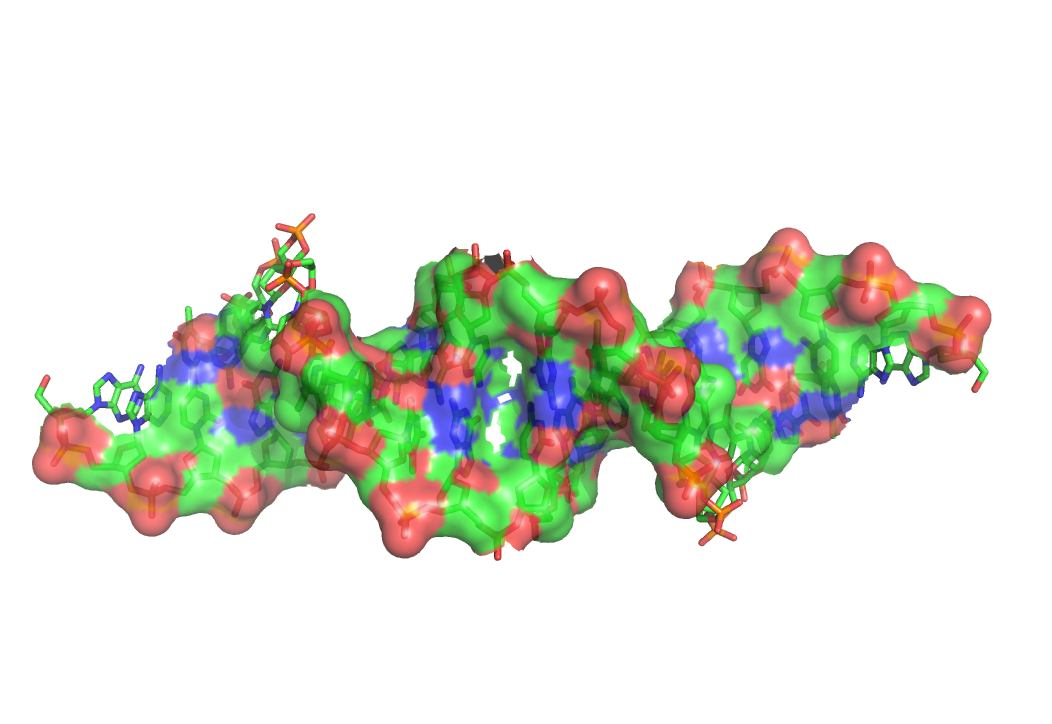
\includegraphics[height=0.8\textheight]{contact-dna.jpg}
    \end{frame}

    \begin{frame}{Ссылки}
        При подготовке данной презентации были использованы материалы с
        сервера компьютерного класса ФББ, Pymol Wiki, Wikipedia, msg.ucsf.edu.
    \end{frame}

\end{document}

